\Chapter{Kiterjesztett és virtuális valóság}

A fejezet a kiterjesztett és a virtuális valóság fogalomrendszerét és eszközkészletét mutatja be.
Mindkettő közismert fogalomnak tekinthető, sok hasonlóságot mutatnak, mégis koncepcionális különbségek vannak közöttük.
A következőkben ezek tisztázására kerül sor.

\Section{Alapfogalmak}

A témakör fogalomrendszere az alábbi három megközelítés köré épül.
\begin{itemize}
\item[AR] (\textit{Augmented Reality}):
A kiterjesztett vagy augmentált valóság alatt a valóság kibővítését értjük. Ehhez valamilyen eszköz kameráján keresztül kell szemlélnünk a teret. Fontos kiemelni, hogy az augmentálás azt jelenti, hogy a valós képre kerülnek rá a plusz elemek.
\item[VR] (\textit{Virtual reality}): A virtuális valóság, a valóság teljes kizárása és egy virtuális környezetbe kerülést jelent. (Eszközkészletében megjelenhetnek azonban olyan elemek, amelyek a valóságos térből kapott információk segítségével teszik módosíthatóvá a virtuális teret. Ilyenek például a különböző elmozdulásszenzorok.)
\item[MR] (\textit{Mixed Reality}): Az AR és VR keveréke. A valós teret bővíti ki, ahogy az AR, azonban itt a cél a virtuális és valós környezet határának elmosása. Nagyobb hangsúlyt kap az interakció. 
\end{itemize}

\Section{Hardver elemek}

\SubSection{AR hardverek}

Ahhoz, hogy ízelítőt kapjuk a kiterjesztett valóság használatának élményéből elegendő egy megfelelő operációs rendszerrel rendelkező mobiltelefon vagy tablet.
Android 7-től, iOS 11-től már számos alkalmazás (többségében játék) érhető el, amelyek nem igényelnek további speciális eszközöket. 

Ezek az okos eszközök azért felelnek meg erre a célra, mert rendelkeznek kamerával.
Az újabb telefonok már igen éles és tiszta kameraképet adnak, és további olyan szenzorokkal is felszerelték őket, amelyek alkalmassá teszik őket a valóság kiterjesztéséhez.

Ezen érzékelők  mikro-elektromechanikai (MEMS, \textit{Micro Electro Mechanical Systems}) 
rendszerek, azaz olyan apró (karakterisztikus méretük jellemzően 20\-1000 mikrométer) rendszerek, amelyek mechanikai és elektronikai alkatrészeket is tartalmaznak \cite{mems}.

A telefonok jellemzően a következő MEMS szenzorokat tartalmazzák:
\begin{itemize}

\item {\bf Gyorsulásérzékelő} (accelerometer): Az eszközre ható gyorsulást igyekszik mérni. Ezt az eszközre hatókból tudja becsülni (Newton 2. törvényének megfelelően az $F = m \cdot a$ összefüggésből) \cite{gyorsulas}.
\item {\bf Giroszkóp}: Szögben történő elfordulást és annak sebességét méri/becsli \cite{giroszkop}.
\item {\bf Inerciális szenzor}: accelerometer és giroszkóp együttese.
\item Fontos érzékelő még a távolságérzékelő, iránytű, fényváltozás érzékelő.
\end{itemize}

Az asztali számítógépek valamint laptopok is használhatók kiterjesztett valósághoz, ha el vannak látva kamerával.

% A Unity legújabb verziói (2019.3-tól sé annál frissebb) már nem csak a Windows-t és MacOS támogatják, hanem  lehetővé teszik a Linux operációs rendszerekre való fejlesztést is.

Az AR eszközökön belül egy speciális kategóriát képviselnek a \textit{headset}-ek.

2019 legnépszerűbb AR headsetjei a következők.
\begin{itemize}
\item {\bf Microsoft Hololens 2}: Egy vezeték nélküli AR headset, ami két éles kijelzővel rendelkezik, ezért jobb felhasználói élményt bíztosít, mint a versenytársai.

A interakciót a 3D-s objektumokkal a \textit{Holographic Processing Unit} biztosítja, illetve el van látva egy HD kamerával, számos mikrofonnal és fényérzékelővel.

Írányítani a tekintet (a virtuális elemek megjelenítéséhez használt kamerapozíciót), fejmozgás és a testmozgás segítségével lehet.

Az eszközről egy képet \aref{fig:hololens}. ábrán láthatunk.

\item {\bf MagicLeap One}: Egy igazán futurisztikus kinézettel rendelkező AR headset.

Szintén lehetőség van a kivetített objektumokkal való interakciókra, azonban a \textit{Hololens}-szel ellentétben nem a felhasználó mozgása, hanem egy kontrollel valósítja meg ezt. 

Egy igen kisméterű számítógép felel a interakció további megvalósításáért, ami a \textit{Lightpack} nevet viseli (tehát nem vezeték nélküli).
  
\item {\bf Epson Moverio}: kifejezetten munkára tervezetett AR headset, ezért robosztus kialakításasal rendelkezik.

Az \textit{Epson Moverio} által felhasznált Si-Oiled technológia tiszta, éles képet bíztosít a felhasználó számára.

A hozzá tartozó Intel Axom 3 processzorral rendelkezik és az Android 5.1-es verzióját használja. 

A rendszer képes a szemmozgást követni.

\item {\bf Google Glass Enterprise}: Ez nem igényel kontrollert, kéz nélkül használható.
Az Enterprise plusz funkciói a többi Google Glass-hoz képest:
\begin{itemize}
\item hangvezérlés,
\item könnyebb súly,
\item hosszabb akkumulátor élettartam,
\item gyorsabb processzor és 8 MP kamera. \cite{arhardware}
\end{itemize}
\end{itemize}

\begin{figure}[htp]
    \centering
   	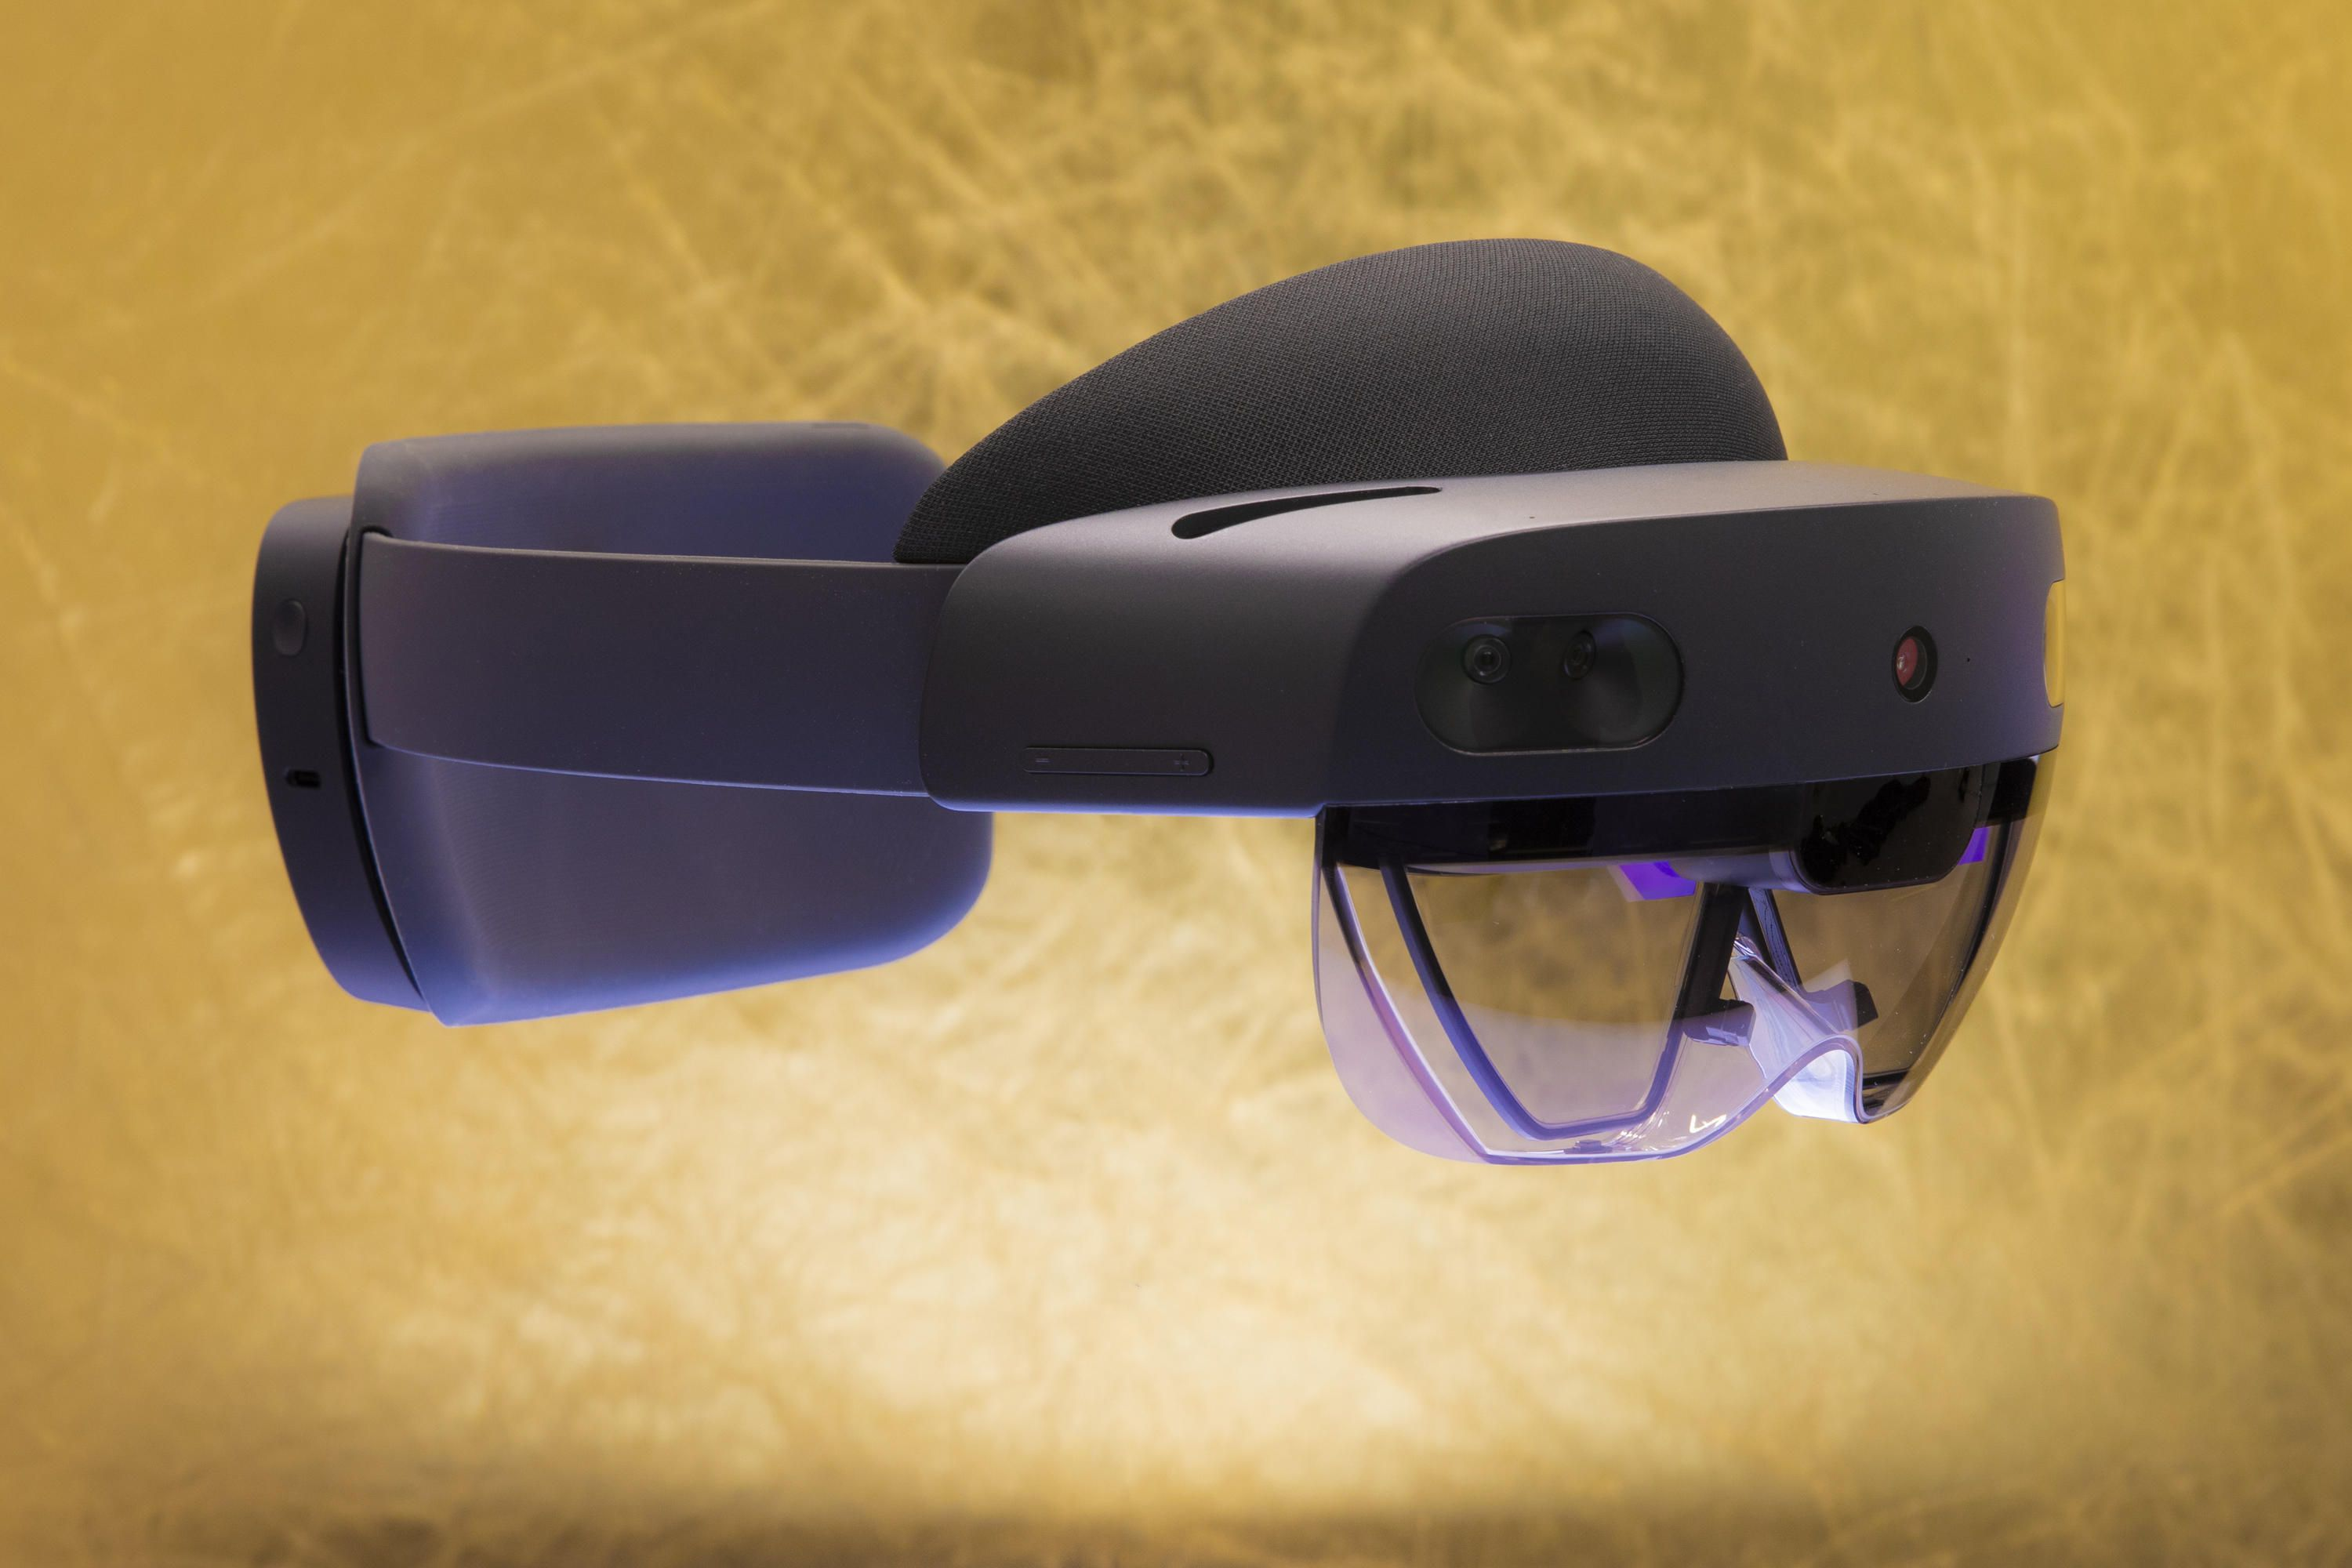
\includegraphics[scale=0.1]{images/holo.jpg}
	\caption{Hololens 2 kiterjesztett valóság szemüveg}
	\label{fig:hololens}
	\cite{hololens}
\end{figure}

Az említett headset-ek kereskedelmi forgalomban kaphatók, ám magas áruk miatt nehezen terjednek. 

\SubSection{VR hardverek}

A virtuális tér kialakításához szükség van megfelelő hardverekre, mint például hangrenszer, kijelző (VR szemüveg), számítógép, telefon, konzol továbbá speciális szenzorok, amelyek követik a felhasználó mozgását (test, kéz, fej).

A következőket tekinthetjük a dolgozat megírásának idejében a leginkább elterjedt VR eszközöknek.
\begin{itemize}
\item {\bf Valve Index}: Remekül működik régebbi GPU esetén is, éles kijelzővel rendelkezik és a Valve kontroller képes az összes ujj mozgását követni. Azonban nehéz kalibrálni és beállítani. A magasabb árkategóriába tartozik.
\item {\bf Oculus Quest 2}: Könnyű a használata, azonban Facebook fiók hozzáadást igényel. \Aref{fig:occulus}. ábrán láthatunk róla egy képet.
\item {\bf PlayStation VR}: PS4 konzol szükséges hozzá. Sok játék elérhető hozzá. Nem a legjobbb a mozgás követésének a tekintetében.
\item {\bf Oculus Rift S}: Nem vezeték nélküli, így korlátoltabb a mozgás tér.  Kényelmesebb, mint az előző verziója, micwl könnyű. Viszonylag sok játék érhető el hozzá.
\item {\bf Samsung Gear VR}: Samsunk okostelefonnal használható (Galaxy S8-tól felfelé) \cite{vrheadset}.
\end{itemize}

\begin{figure}[htp]
    \centering
   	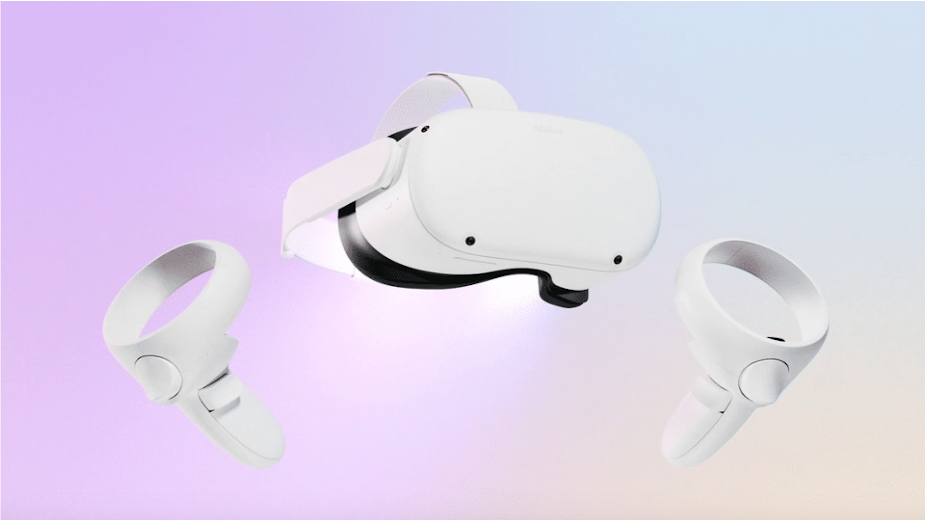
\includegraphics[scale=1]{images/oculus.png}
	\caption{Oculus Quest 2 virtuális valóság szemüveg és a hozzá tartozó vezérlők\cite{occulus}}
	\label{fig:occulus}
\end{figure}

A következőkben néhány népszerű kontroller kerül említésre.
\begin{itemize}
\item \textbf{HTC Vive}: Képes követni a kéz mozdulatot, az ujjak mozgását.
\item \textbf{3DRudder}: Lábbal vezérelhető.
\item \textbf{SteelSeries Stratus XL}: Konzolhoz való kontroller kialakítású \cite{kontroller}.
\end{itemize}

A VR kesztyűk egy külön alkategóriát képviselnek.
Precízebben lehet velük követni a kéz mozgását, külön követik a ujjak mozgását.
Ilyenek például az \textit{ExoGlove}, \textit{ManusVR} és a \textit{GloveOne} (\ref{fig:gloveone}. ábra).

\begin{figure}[htp]
    \centering
   	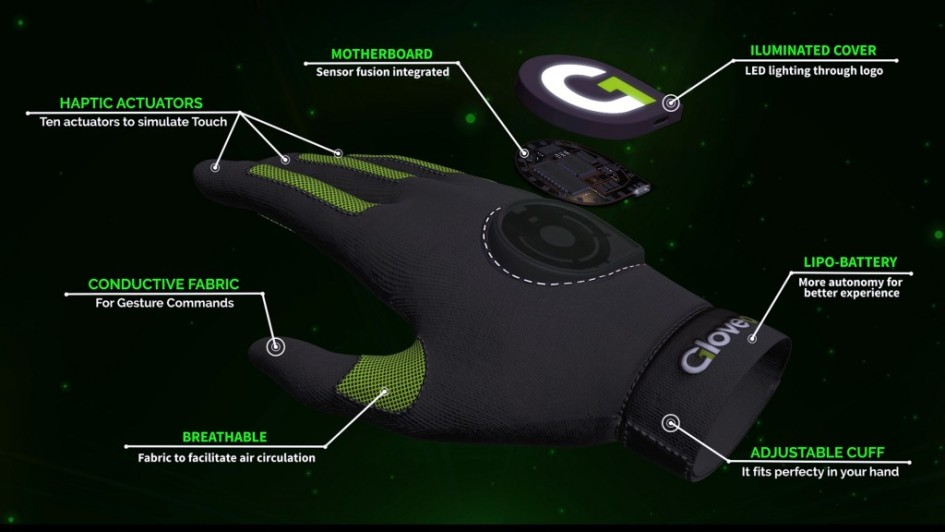
\includegraphics[scale=0.6]{images/gloveone.jpg}
	\caption{OneGlove VR kesztyű \cite{gloveOne}}
	\label{fig:gloveone}
\end{figure}

Érdekességképpen érdemes még megemlíteni a VR ruhákat, amelyek megpróbálják a lehető legközelebb hozni a felhasználót a virtuális térben lévő elemekhez.
Ilyen eszközök például a \textit{TeslaSuit} (\ref{fig:teslasuit}. ábra)) és a \textit{TactSuit}.

\begin{figure}[htp]
    \centering
   	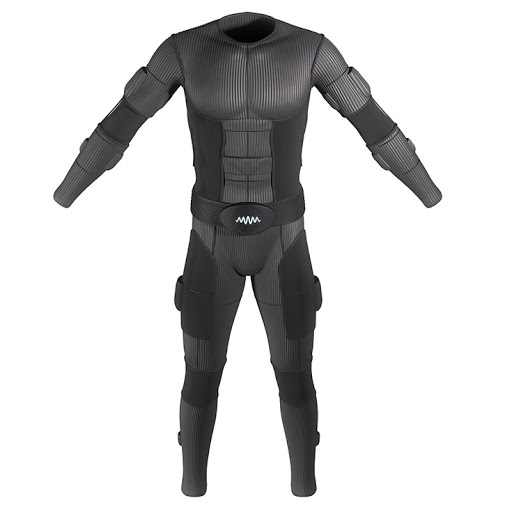
\includegraphics[scale=0.3]{images/tesla.jpg}
	\caption{TeslaSuit VR ruha \cite{tesla}}
	\label{fig:teslasuit}
\end{figure}

\Section{A kiterjesztett valóság fajtái}

\SubSection{Marker alapú megoldások}

A markerek speciális azonosítók, amelyeket kamera segítségével, az AR alkalmazással felismerünk és a virtuális tartalmat (ami lehet egy  3D objektum például), a kamerához vizsonyított relatív pozicióba helyezzük el. 

Fontos, hogy a marker egyedi legyen és jól felismerhető a környezetben. 

Hátránya, hogy ha a marker egy része nem látható (például annak hatására, ha az eszköz elmozdul) akkor a tartalom eltűnik.
Marker lehet egyszerűbb információt hordozó bináris minta kerettel (például QR-kód vagy ArUco marker), síkbeli vagy térbeli objektum is.

\SubSection{Marker nélküli megoldások}

A marker nélküli kiterjesztett valóság jellemzően SLAM-et (\textit{Simultaneous Localization and Mapping}) használ környezet felmérése és követésére.
Érzékelheti például, hogy hol a padló, a plafon vagy a falak.
A megjelenített tartalmakat így a környezethez lehet viszonyítani, tájolni.

Lényeges elönye, hogy a virtuális tartalom itt nem tűnik el elmozdulás miatt, hisz nem egy adott markerhez,
hanem az egész környezethez számítja az alkalmazás annak pozícióját.

\Section{Szoftverek, fejlesztőeszközök}

A következőkben az elterjedt szoftveres eszközkészletek bemutatására kerül majd sor.

\SubSection{Apple ARKit}

Az Apple ARKit az iOS operációs rendszerrel (iOS 11-től felfelé) rendelkező eszközökre (iPhone, iPad amiknek minimum A9-es processzora van) való AR alkalmazások fejlesztéséhez használható. 
Például képes: 
\begin{itemize}
\item 2D-s kép felismerésére és annak követésére,
\item 3D-s objektum felismerésére és annak elhelyezésére a térben.
\item Az újabb verziókkal többjátékos módot támogató játékok készíthetők. 
\end{itemize}

\SubSection{Google ARCore}

A \textit{Google ARCore} igen népszerű AR SDK. Használható tabletre, telefonra való iOS és Android alkalmazások készítéséhez. Az SDK alapját a pozició követés és az objektum felismerés jelenti.
Fontos elemei az alábbiak.
\begin{itemize}
\item A fény követés a valósághűbb objektumok megjelenítéséhez.
\item Mozgás követés a telefon poziciójának felhasználásával.
\item Felismerése a felületek abszolút méretének, elhelyezkedésének függőlegesen és vízszintesen.
\end{itemize}

\SubSection{Vuforia}

A \textit{Vuforia} az egyik legnépszerűbb SDK a AR alkalmazások készítéséhez.

Annak köszönhetően, hogy \textit{Unity}-ben jól használható, lehetővé válik vele a Android-ra és iOS-re való natív alkamazások készítése (számos programozási nyelvet használva).

Asztali gépekre is lehet vele fejleszteni, szintén a Unity-nek köszönhetően. 
  
A következők a jellegzetes funkciói.
\begin{itemize}
\item  Kép, (angol nyelvű) szöveg, 3D-s objektumok felismerése és követése valós időben.
\item  Virtuális elemek elhelyezése a térben.  
\item  Virtuális gombok.
\item  Lokalizált okklúzió felismerés a virtuális gombok használatával.
\end{itemize}
Használható számos marker típussal, marker nélkül, markerként használt objektumokkal, \textit{VuMark}-kal (amely a QR-kód és kép együttese).

\SubSection{Wikitude}

A \textit{Wikitude} kíválóan alkalmazható hely-központú( WIFI vagy GPS felhasználásával) alkalmazások fejlesztésére telefonra. 

Népszerű az ipari felhasználás területén, annak köszönhetően, hogy a legrövidebb idő alatt ezzel lehet elkészíteni a vásárló-központú alkalmazásokat. 

Fő funkciói az alábbiak:
\begin{itemize}
\item 3D, kép felismerés és követés,
\item helymeghatározáson alapuló AR,
\item okos szemüveg integráció.
\end{itemize}

\SubSection{Kudan}

A \textit{Kudan} egy réteget add hozzá az objektumokhoz a felismerés megkönnyítése végett. Gyors és egészen egyszerű a használata. 
Használható markerrel és marker nélkül is.

\SubSection{ARToolKit}

Az \textit{ARToolKit} nyílt forráskodú (elérhető GitHub-on). Használható akár okosszemüvegekhez készített alkalmazások fejlesztéséhez is. Fejleszhető vele iOS, Android, Windows, MacOS és Linux platformra is alkalmazás. 
Rendelkezik \textit{Unity} és \textit{OpenSceneGraph} támogatással.
Megvalósítja az egy vagy duálkamerával való követést. Számos programozási nyelvvel használható.

\SubSection{EasyAR}

Az \textit{EasyAr} ingyenes, kiváló szoftveres eszköz kezdőknek. Van professzionális verziója is üzleti használatra, amely extra funkciókat tartalmaz. Androidra, iOS-re és Windows-ra van lehetőség fejleszteni vele.

\SubSection{MaxST}

A \textit{MaxST} két SDK-ra válik szét: egy a 2D kép felismeréshez, és egy a 3D objektumokhoz.
Felismeri a függőleges és vízszintes síkokat, így akár több objektumot is képes egyszerre követni. Alkalmas QR-kód és vonalkód szkenneléshez.

\SubSection{Pikkart AR SDK}

A \textit{Pikkart} SDK segítségével egyedi, funkció gazdag, felhasználóbarát alkallmazásokat lehet készíteni. Könnyű fejlesztési folyamatot biztosít.

\SubSection{AR.js}

Az \textit{AR.js} egy JavaScript alapú, nyíltforráskodú AR SDK. Böngészőben használható AR alkalmazások készítéséhez. Nem igényel semmilyen telepítést. Minden mobil platformon képes futni az ezzel az SDK-val készített alkalmazás.

\SubSection{További API-k}

Számos további API is elérhető. Név szerint említés szintjén például a következők:
\begin{itemize}
\item ARLab,
Onirix,
DeepAR,
MixedReality Toolkit (Hololens),
Xzimg,
DroidAR,
HP Reveal Studio,
BlippBuilder \cite{arsdks}.
\end{itemize}

\Section{Unity}

A \textit{Unity} egy  olyan keresztplatformos játékmotor, amellyel lehetőségünk van Windows-ra, Linux-ra, Mac OS-re, iOS-re, Android-ra, valamint Wii-re és más játék konzolokra fejleszteni.

Van üzleti és személyi változata is. Bizonyos keretek alatt ingyenes lehet a cégeknek is, nem csak a magánszemélyeknek.

A hozzáférhető leírások alapján először a \textit{Unity} keretrendszer tünt megfelelőnek a dolgozatban bemutatott program elkészítéséhez.
A későbbiekben azonban számos probléma lépett fel, mint például a következők.
\begin{itemize}
	\item Túlságosan erőforrás igényes, speciális eszközöket igényelnek a kiprobálható demók (pl. VR szemüveg).
	\item A különböző verziókhoz tartozó leírásokban nehéz kiigazodni. Az adott problémákhoz fellelhető megoldások csak az adott verzión működtek.
\end{itemize}

\Section{Alacsonyabb szintű eszközök integrációja}

A korábban bemutatott, igen változatos és funkciókban gazdag eszközkészlet számos problémát hordozott magában.
Ezen okok miatt a fejlesztést egyszerűbb, de stabilan működő függvénykönyvtárak integrációjával tünt célszerűnek megoldani.
\begin{itemize}
	\item \textit{OpenCV}: Gépi látáshoz használt függvénykönyvtár.
	\item \textit{OpenGL}: Nyílt grafikus nyelv és a hozzá tartozó függvénykönyvtár.
\end{itemize}
A Python programozási nyelv alkalmasnak bizonyult arra, hogy ezek funkcióihoz egyszerűen hozzá lehessen férni, azokat egy alkalmazásba könnyen lehessen integrálni.
